\section{Performance Analysis}

There are some other proposed solutions in this field \citep{osvik,paladi,rudra2001efficient,matsui2006far,matsui2007power,konighofer2008fast,meushaw2005device}. We take some of the most prominent ones and compare it with our proposed solution.\\

\paragraph{Avoiding Memory Access}
Since the cache-timing attacks exploit the effect of memory access on the cache, any implementation that does not perform any table lookup won't suffer from this sort of attacks. But it has a major drawback. The performance is degraded by an order of magnitude. We need a total of 24 shift operations, 16 table lookups, 8 conditional XOR operations, 28 mandatory XOR operations for a single round in a straightforward implementation.\\

In fact, the conditional XOR operation is vulnerable to timing attack too \citep{stallings5}. Other than lagging behind in terms of security, straightforward implementation requires more computation time. But the positive side is, straightforward implementation doesn't need to maintain any sort of lookup table other than the S-Box. On the other hand, table lookup with RAT has an overhead of mapping and inverse mapping during encryption. From algorithm 5 it is prominent that a single call to inverse mapping function incurs 4 shift operations, 3 AND operations, 2 addition operations on a single integer. This has very intangible effect on small amount of data. But when plain text becomes very large, the difference becomes clear.\\

Encrypting as much as 80 Mega Bytes of plain text required 12.3 seconds for a normal table lookup approach whereas the same operation required 52.1 seconds for a RAT assisted approach on the same platform. So it turns out that, the proposed approach is approximately 300\% slower than a normal approach. In other words, encrypting 1 Byte requires 4 times more time than a regular approach. In real time, we hardly need to encrypt bulk volume of data. Novertheless, RAT is impractical for cases where we really need to encrypt excess amount of data.\\

\paragraph{Disable Cache Sharing}
To protect against software-based attacks, it would suffice to prevent cache state effects from spanning process boundaries. But practically this is very expensive to achieve. On a single threaded processor, it would require flushing the whole cache during every context switch. On a multi threaded processor, it would also require the logical processors to use separate logical caches, statically allocated within the physical cache; some modern processors do not support such a mode \citep{osvik}. Using RAT will not impose any restriction about cache sharing which is perfectly suitable for cloud environment and virtual machines (without causing evictions and filling).

\begin{center}
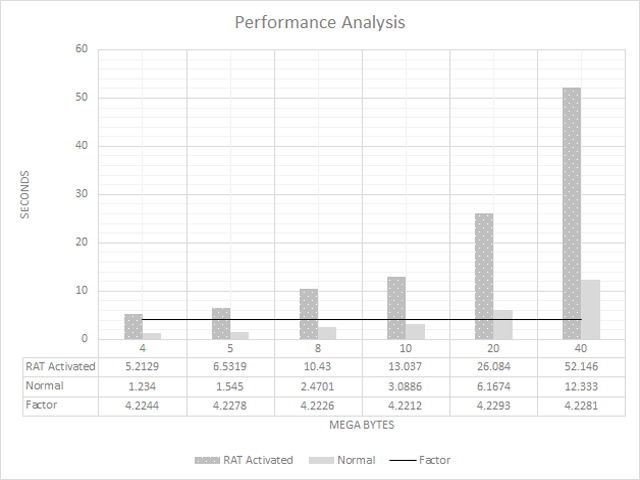
\includegraphics[scale=0.6,natwidth=640,natheight=480]{psd/performance_analysis.png}
\captionof{figure}{Performance analysis of AES implementations with (dotted column) and without (solid column) the assistance of Random Address Translator in the same platform. Due to mapping overhead, a RAT assisted implementation is 4.2 times slower than a regular table lookup approach. The straight line indicates that this slowing factor doesn't depend on volume of data to be encrypted.}
\end{center}

\paragraph{Static or Disabled Cache}
One brutal countermeasure against the cache-based attacks is to completely disable the CPU's caching mechanism. Of course, the effect on performance would be devastating. A more attractive alternative is to activate a ``no-fill" mode where the memory accesses are serviced from the cache when they hit it, but accesses that miss the cache are serviced directly from the memory. The steps are:

\begin{enumerate}
\item Preload the AES tables into the cache
\item Activate the ``no-fill" mode
\item Perform encryption
\item Deactivate the ``no-fill" mode
\end{enumerate}

The section spanning (1) and (2) is critical, and attacking process must not be allowed to run during this time \citep{osvik}. However, the major drawback of this approach is that, during the encryption process the overall system will be slowed down by a factor since cache access is limited during the encryption process. But using RAT, the ``no-fill" mode is not required. All the other processes can be allowed to access the cache even during the encryption proceeds. To get the best result, the mapping integers should be registered.\\

\paragraph{Dynamic Table Storage}
The cache-based attacks observe memory access patterns to learn about the table lookups. Instead of eliminating these, we may try to decorrelate them. For example, one can use many copies of each table, placed at various offsets in memory, and have each table lookup use a pseudorandomly chosen table. Somewhat more compactly, one can use a single table, but pseudorandomly move it around memory several times during each encryption \citep{osvik}. But the major drawback of this approach is that, it will incur cache misses more than ever. This implies that the encryption process will be slowed down by a large factor. More importantly the performance and security of this approach would become architecture dependent. Using RAT helps us alleviate this situation by obviating the need of moving around the Lookup table in the memory.

Some important benefits of using RAT are
\begin{itemize}
\item The integrity of AES is maintained even though the implementation becomes a client dependent process. There is no need to worry about how other ends of the terminals are encrypting their data.

\item No need of NOP operation. NOP operations are introduced to scramble uniform patterns in various fields. In case of cache-timing analysis, NOP operation would mean accessing Lookup table entry, but doing no operation with it.

\item No need to introduce disturbance in plaintext. Sometimes plaintext is modified before it is passed to the encrypting process. This sort of approach is not suitable for large scale application where the interface must be kept as simple as possible.

\end{itemize}
